\documentclass{article}

\usepackage[english]{babel}
\usepackage[utf8]{inputenc}
\usepackage{amsmath}
\usepackage{amsthm}
\usepackage{amssymb}
\usepackage{amsfonts}
\usepackage{graphicx}
\usepackage{wrapfig}
\usepackage{bbm}
\usepackage{dsfont}

% set up margin
\usepackage
[
  a4paper,
  left=3cm,
  right=3cm,
  top=3cm,
  bottom=3cm,
]
{geometry}

% set up header
\usepackage{fancyhdr}
\pagestyle{fancy}
\fancyhf{}
\lhead{6.438 Algorithms for Inference}
\chead{Problem Set 2}
\rhead{Hongzi Mao}
\cfoot{\thepage}
\rfoot{\footnotesize{\emph{Collaborated with: Hongzhou Ye, Zhiwei Ding}}}

% footer line
\renewcommand{\footrulewidth}{0.4pt}

% sans serif italic
\newcommand{\s}[1]{\textsf{\textit{#1}}}

% set symbol
\usepackage[mathscr]{euscript}

% empty set
\let\emptyset\varnothing

% qed
\newcommand{\qeds}{\hfill\qedsymbol}

% independence symbol
\makeatletter
\newcommand*{\indep}{%
  \mathbin{%
    \mathpalette{\@indep}{}%
  }%
}
\newcommand*{\nindep}{%
  \mathbin{%                   % The final symbol is a binary math operator
    \mathpalette{\@indep}{\not}% \mathpalette helps for the adaptation
                               % of the symbol to the different math styles.
  }%
}
\newcommand*{\@indep}[2]{%
  \sbox0{$#1\perp\m@th$}%        box 0 contains \perp symbol
  \sbox2{$#1=$}%                 box 2 for the height of =
  \sbox4{$#1\vcenter{}$}%        box 4 for the height of the math axis
  \rlap{\copy0}%                 first \perp
  \dimen@=\dimexpr\ht2-\ht4-.2pt\relax
  \kern\dimen@
  {#2}
  \kern\dimen@
  \copy0 %                       second \perp
} 
\makeatother

%%%%%%%%%%%%%%%%%%%%%%%%%%%%%%%%%%%%%%%%%%%%%%%%%%%%%%%%%%%%%%%%%%%%%%%%
%%%%%%%%%%%%%%%%%%%%%%%%% Begin document here %%%%%%%%%%%%%%%%%%%%%%%%%%
%%%%%%%%%%%%%%%%%%%%%%%%%%%%%%%%%%%%%%%%%%%%%%%%%%%%%%%%%%%%%%%%%%%%%%%%
\begin{document}
 
\section*{Problem 2.2}
%
(a) To prove the largest clique size in $\mathscr{H}$ is $\max_i |\mathscr{S}_i| +1$,
we show 
\begin{enumerate}
	\item at every elimination step $i$, the newly generated edges and the eliminated edges to node $i$ forms a clique in $\mathscr{H}$;
	\item such clique has size $|\mathscr{S}_i| +1$; and
	\item the largest clique formed at the eliminated steps is no smaller than the largest clique in the reconstituted graph $\mathscr{H}$.
\end{enumerate}
%
\begin{figure}[h]
  \centering
  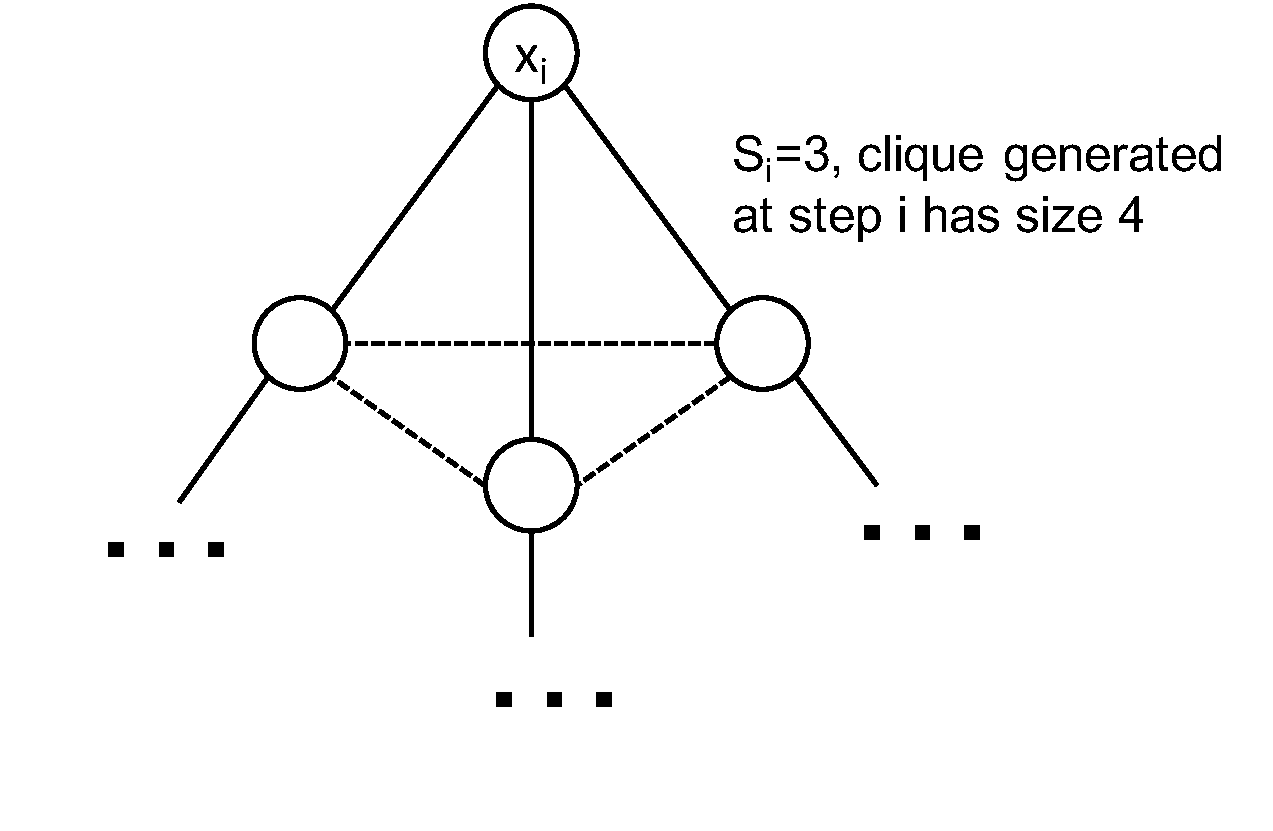
\includegraphics[width=0.5\columnwidth]{2a.pdf}
  \vspace{-0.7cm}
  \caption{Eliminating node $i$.}
  \label{f:2a}
\end{figure}
%

To show (1), we note that nodes in $\mathscr{S}_i$ are fully connected (dashed line in Figure~\ref{f:2a}) at
elimination step $i$ (direct consequence of elimination). Since node $i$ was connected to all nodes in
$\mathscr{S}_i$ (solid line connected to $i$ in Figure~\ref{f:2a}), this nodes set forms a clique.
%
For (2), the size of such clique at each step $i$ is all the uneliminated nodes connected to $i$ and node $i$
itself, i.e., $|\mathscr{S}_i| +1$.

%
To show (3), we first notice that the largest clique formed at elimination steps is no smaller than the largest
clique in the \emph{original} graph $\mathscr{G}$. This is because, at the first time we eliminate any node $j$
in the largest clique of $\mathscr{G}$, the size $|\mathscr{S}_j|$ is at least the clique size $-1$ (as $j$ can
only be connected with more nodes than all the nodes in the clique).

%
Second, the cliques with newly generated edges in $\mathscr{G}$ are formed in single elimination steps. This
can be proved by contradiction. Suppose a clique in $\mathscr{G}$ is formed in multiple elimination steps. In
such a clique, there exists a node \emph{not} connecting to all other nodes in the clique at its elimination
step (otherwise a single step would have formed the clique). But after eliminating this node, other nodes have
no way to form a connection with it, and thus can not form a clique with this node, which is a contradiction.
Thus the largest clique in $\mathscr{H}$ is generated in a \emph{single} elimination step.

Therefore, the largest clique generated at the elimination steps, i.e., with size $\max_i |\mathscr{S}_i| +1$,
is the largest clique in $\mathscr{H}$. \qeds
\\

%
\noindent
(b) We show $\mathscr{H}$ is chordal by induction.
%
For any cycle in $\mathscr{H}$ of size $4$, when eliminating any of the node will add in an edge (if not already
exist) between its adjacent nodes, which makes makes this cycle chordal in $\mathscr{H}$.

%
Assume any cycle in $\mathscr{H}$ with size $N$ or less is chordal. For a cycle in $\mathscr{H}$ with size $N+1$,
if there are existing edges connecting any nodes in the cycle, the cycle can be decomposed into multiple cycles
with size strictly less than $N+1$. For all these cycles, they are chordal since their sizes are $N$ or less. If
there is no previous edge in the cycle, eliminating any node will connect its adjacent nodes, making a triangle
and a cycle with size $N$. Since the cycle with size $N$ in $\mathscr{H}$ is chordal and the triangle connects
the 2 non-consecutive edges are connected in the triangle, the cycle with size $N+1$ is chordal. 

%
Therefore, by induction, $\mathscr{H}$ is chordal. \qeds

\pagebreak

%%%%%%%%%%%%%%%%%%%%%%%%%%%%%%%%%%%%%%%%%%%%%%%%%%%%%%%%%%%%%%%%%%%%%%%%%%%%%%%%%%%%%%%%
\section*{Problem 2.3}
(a) Figure~\ref{f:3a} shows the reconstituted graph.
%
\begin{figure}[h]
  \centering
  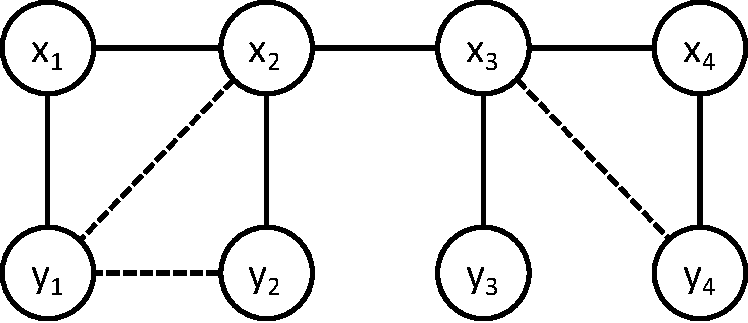
\includegraphics[width=0.4\columnwidth]{3a.pdf}
  \vspace{-0.2cm}
  \caption{Reconstituted graph induced by elimination ordering $(\s{x}_4,\s{y}_4,\s{y}_3,\s{x}_3,\s{x}_1,\s{x}_2,\s{y}_2,\s{y}_1)$.}
  \label{f:3a}
\end{figure}
%
\\

%
\noindent
(b) An elimination ordering that requires the least computation:
$(\s{y}_1, \s{y}_2, \cdots, \s{y}_n, \s{x}_1, \s{x}_2, \cdots, \s{x}_n)$.
%
The asymptotic time complexity is $O(nk^2)$.
%
This is the least computation because every elimination step does not introduce new edge, every step takes
the least $O(k^2)$ computation, and there are $2n$ nodes to eliminate at least.

An elimination ordering that requires the most computation:
$(\s{x}_1, \s{x}_2, \cdots, \s{x}_n, \s{y}_1, \s{y}_2, \cdots, \s{y}_n)$.
%
The asymptotic time complexity is $O(k^{n+1})$. This is the most computation because when eliminating node $\s{x}_n$,
it has connected to all $\s{y}_1, \s{y}_2, \cdots, \s{y}_n$ nodes (i.e., $|\mathscr{S}_{\s{x}_n}| = n$). In this ordering,
if we had eliminated any $\s{y}_i$ before eliminating all $\s{x}$'s, $|\mathscr{S}_{\s{x}_n}|$ would have been less than
$n$; and the ordering among $\s{x}$ does not matter because eliminating some middle $\s{x}_i$ first does not increase the
connectivity in terms of $\s{x}$'s for its adjacent $\s{x}_{i-1}$ and $\s{x}_{i+1}$ when eliminating them (i.e., $|\mathscr{S}_{\s{x}_{i-1}}| \leq n$ and $|\mathscr{S}_{\s{x}_{i+1}}| \leq n)$.
%
\\

%
\noindent
(c) Figure~\ref{f:3c} shows an example.
%
\begin{figure}[h]
  \centering
  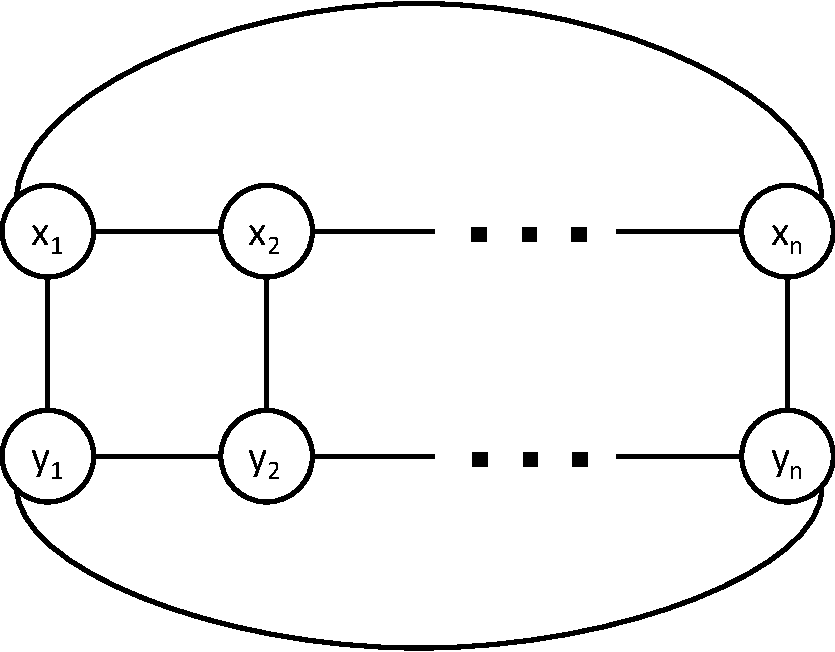
\includegraphics[width=0.4\columnwidth]{3c.pdf}
  \vspace{-0.1cm}
  \caption{An example of undirected graph that the maximal clique size does not dependent on $n$ (maximal cliques
  are edges, size $2$). The elimination complexity of any ordering is $O(k^{n/2})$.}
  \label{f:3c}
\end{figure}
%
\pagebreak

%%%%%%%%%%%%%%%%%%%%%%%%%%%%%%%%%%%%%%%%%%%%%%%%%%%%%%%%%%%%%%%%%%%%%%%%%%%%%%%%%%%%%%%%
\section*{Problem 2.4}
%
(a)
%
We use sum-product algorithm to pass message from $\s{t}$ to $\s{x}$. Thus
\begin{align*}
m_{\s{t}}(\s{x}=1) &= \sum_t \phi_{\s{t}}(t)\psi_{\s{t}\s{x}}(t, \s{x}=1) \\
&= \sum_t p_{\s{t}}(t)c_{t}.
\end{align*}
%
The margin is then
\begin{align*}
p_{\s{x}}(1) &\propto \phi_{\s{x}}(\s{x}=1) m_{\s{t}}(\s{x}=1)\\
&= \sum_t p_{\s{t}}(t)c_{t},\\
\end{align*}
%
which is automatically normalized since $p_{\s{x}}(0) \propto \sum_t p_{\s{t}}(t)(1-c_{t})$. 
%
Thus,
\begin{equation*}
p_{\s{x}}(1) = \sum_t p_{\s{t}}(t)c_{t}.
\end{equation*}
\\

%
\noindent
(b) 
For ease of explanation, denote the observation of $\s{\textbf{y}}$ to be $\textbf{a} = (a_1, a_2, \cdots, a_N)$.

%
When observation $\s{\textbf{y}} = \textbf{a}$ is given, we can update the graph by updating the singleton
potential on $\s{y}_i$'s to be
\begin{equation*}
	\phi'_{\s{y}_i}(y_i) = \mathds{1}_{y_i = a_i}.
\end{equation*}

To get $p_{\s{x}|\s{\textbf{y}}}(1|\textbf{a})$, we use sum-prodct algorithm to choose $\s{x}$ as root and pass
messages from $\s{y}_i$'s to $\s{t}$ and to $\s{x}$. Specially,
%
\begin{align*}
	m_{\s{y}_i\to\s{t}}(t) &= \sum_{y_i} \psi_{\s{t},\s{y}_i}(t, y_i) \phi'_{\s{y}_i}(y_i)\\
	&=\sum_{y_i} \frac{\exp(\theta^t_iy_i)}{1 + \exp(\theta^t_iy_i)} \mathds{1}_{y_i = a_i}\\
	&=\frac{\exp(\theta^t_i a_i)}{1 + \exp(\theta^t_i)}.
\end{align*}

Next, the message from $\s{t}$ to $\s{x}$ is

\begin{align*}
	m_{\s{t}\to\s{x}}(x=1) &= \sum_{t=1}^K \phi_{\s{t}}(t) \psi_{\s{t,x}}(t, x) \prod_{i=1}^{N} m_{\s{y}_i\to\s{t}}(t)\\
	&=\sum_{t=1}^K p_{\s{t}}(t)c_t\prod_{i=1}^{N}\frac{\exp(\theta^t_i a_i)}{1 + \exp(\theta^t_i)}.
\end{align*}
%

Hence, since $\phi_{\s{x}}(x)=1$,
\begin{align*}
p_{\s{x}|\s{\textbf{y}}}(1|\textbf{a}) \propto \sum_{t=1}^K p_{\s{t}}(t)c_t\prod_{i=1}^{N}\frac{\exp(\theta^t_i a_i)}{1 + \exp(\theta^t_i)}.
\end{align*}

To normalize, notice $p_{\s{x}|\s{\textbf{y}}}(1|\textbf{a}) + p_{\s{x}|\s{\textbf{y}}}(0|\textbf{a}) = 1$ and 
\begin{align*}
p_{\s{x}|\s{\textbf{y}}}(1|\textbf{a}) + p_{\s{x}|\s{\textbf{y}}}(0|\textbf{a}) &= 
\sum_{t=1}^K p_{\s{t}}(t)c_t\prod_{i=1}^{N}\frac{\exp(\theta^t_i a_i)}{1 + \exp(\theta^t_i)} + 
\sum_{t=1}^K p_{\s{t}}(t)(1 - c_t)\prod_{i=1}^{N}\frac{\exp(\theta^t_i a_i)}{1 + \exp(\theta^t_i)} \\
&= \sum_{t=1}^K p_{\s{t}}(t)\prod_{i=1}^{N}\frac{\exp(\theta^t_i a_i)}{1 + \exp(\theta^t_i)}.
\end{align*}

Thus, 
\begin{align*}
p_{\s{x}|\s{\textbf{y}}}(1|\textbf{a}) = \sum_{t=1}^K p_{\s{t}}(t)c_t\prod_{i=1}^{N}\frac{\exp(\theta^t_i a_i)}{1 + \exp(\theta^t_i)} \Bigg/ \sum_{t=1}^K p_{\s{t}}(t)\prod_{i=1}^{N}\frac{\exp(\theta^t_i a_i)}{1 + \exp(\theta^t_i)}.
\end{align*}
\\

%
(c) To use sum-product algorithm, we choose $\s{y}_1$ as root and pass messages to it. Notice that the messages to $\s{t}$,
\begin{align*}
	m_{\s{x}\to\s{t}}(t) &= \sum_x \phi_{\s{x}}(x)\psi_{\s{t, x}}(t, x)\\
	&= \sum_x p_{\s{x}|\s{t}}(x|t)\\
	&=1,
\end{align*}
and
\begin{align*}
	m_{\s{y}_i\to\s{t}}(t) &= \sum_x \phi_{\s{y}_i}(y_i)\psi_{\s{t},\s{y}_i}(t, y_i)\\
	&= \sum_x p_{\s{y}_i|\s{t}}(y_i|t)\\
	&=1.
\end{align*}

Thus, 
\begin{align*}
	m_{\s{t}\to\s{y}_1}(y_1) &= \sum_{t=1}^{K}\phi_{\s{t}}(t)\psi_{\s{t},\s{y}_1}(t, y_1)\\
	&= \sum_{t=1}^{K}p_{\s{t}}(t)\frac{\exp(\theta_1^ty_1)}{1 + \exp(\theta_1^t)}.
\end{align*}

Hence, since  $\phi_{\s{y}_1}(y_1)=1$,
\begin{align*}
	p_{\s{y}_1}(y_1) \propto \sum_{t=1}^{K}p_{\s{t}}(t)\frac{\exp(\theta_1^ty_1)}{1 + \exp(\theta_1^t)}.
\end{align*}

Notice that the probability is automatically normalized, we have
\begin{align*}
	p_{\s{y}_1}(1) = \sum_{t=1}^{K}p_{\s{t}}(t)\frac{\exp(\theta_1^t)}{1 + \exp(\theta_1^t)}.
\end{align*}
%
\pagebreak

%%%%%%%%%%%%%%%%%%%%%%%%%%%%%%%%%%%%%%%%%%%%%%%%%%%%%%%%%%%%%%%%%%%%%%%%%%%%%%%%%%%%%%%%
\section*{Problem 2.5}
%
(a) (i) After stripping off the leaf nodes, the nodes in $G$ that did not have connection to the leaf nodes have their node and edge potentials unmodified. For the nodes that had connection to one or more leaf nodes, their node potentials are updated as
\begin{align*}
	\phi'_\s{s}(s) &= \phi_\s{s}(s) \prod_{\s{t}\in\mathcal{L}(\s{s})}m_{\s{t}\to\s{s}}(s) \\
	&= \phi_\s{s}(s)\prod_{\s{t}\in\mathcal{L}(\s{s})}\sum_{t}\phi_\s{t}(t)\psi_{\s{t}, \s{s}}(t, s),
\end{align*}
where $\mathcal{L}(\cdot)$ denotes the neighboring leaf nodes.
\\

%
(ii) We show $G'$ has diameter strictly less than $D-1$ by showing (1) all the paths in $G$ reduce the length by $2$ and
(2) a path in $G'$ must be fully contained by a path in $G$. 

Here, (1) is because the two ends of a path in $G$ are different (otherwise a cycle in tree), and the two ends are
leaves (otherwise not a path). These two ends are stripped off as they are separate leaves. Thus the length of any path
in $G$ is reduced by 2. 

We show (2) by contradiction. Any two nodes in $G'$ must on a path in $G$, because otherwise the graph is disjoint.
Then we assume a path in $G'$ was not a part of any path in $G$. We can pick any two nodes in path. Now these two nodes
has a path in $G$; we can walk along this path from a node to the other. Then since the path in $G'$ is \emph{different},
we can walk along the path in $G'$ back to the starting node, which forms a cycle. Thus any path in $G'$ must originally
be part of a path in $G$, which completes the second part of this proof. \qeds
\\

%
(iii) We need to show two directions. First, the messages from the leaf nodes were fixed because the messages sent out
from the leaves do not depend on other nodes. Second, by induction step, the messages from "inside" are all converged
by $D-2$ time steps. Therefore, the message sent to the leaves are also fixed. Thus, after "placing back" the leaf nodes
and conduct one more message passing, all the messages will have converged.
\\

%
\noindent
(b) For depth $= 1$ the equation holds, since
\begin{align*}
m_{\s{s}\to\s{t}}^*(x_t) &= \sum_{x_s}\psi(x_s, x_t)\phi(x_s).\\
\end{align*}
%
\begin{figure}[h]
  \centering
  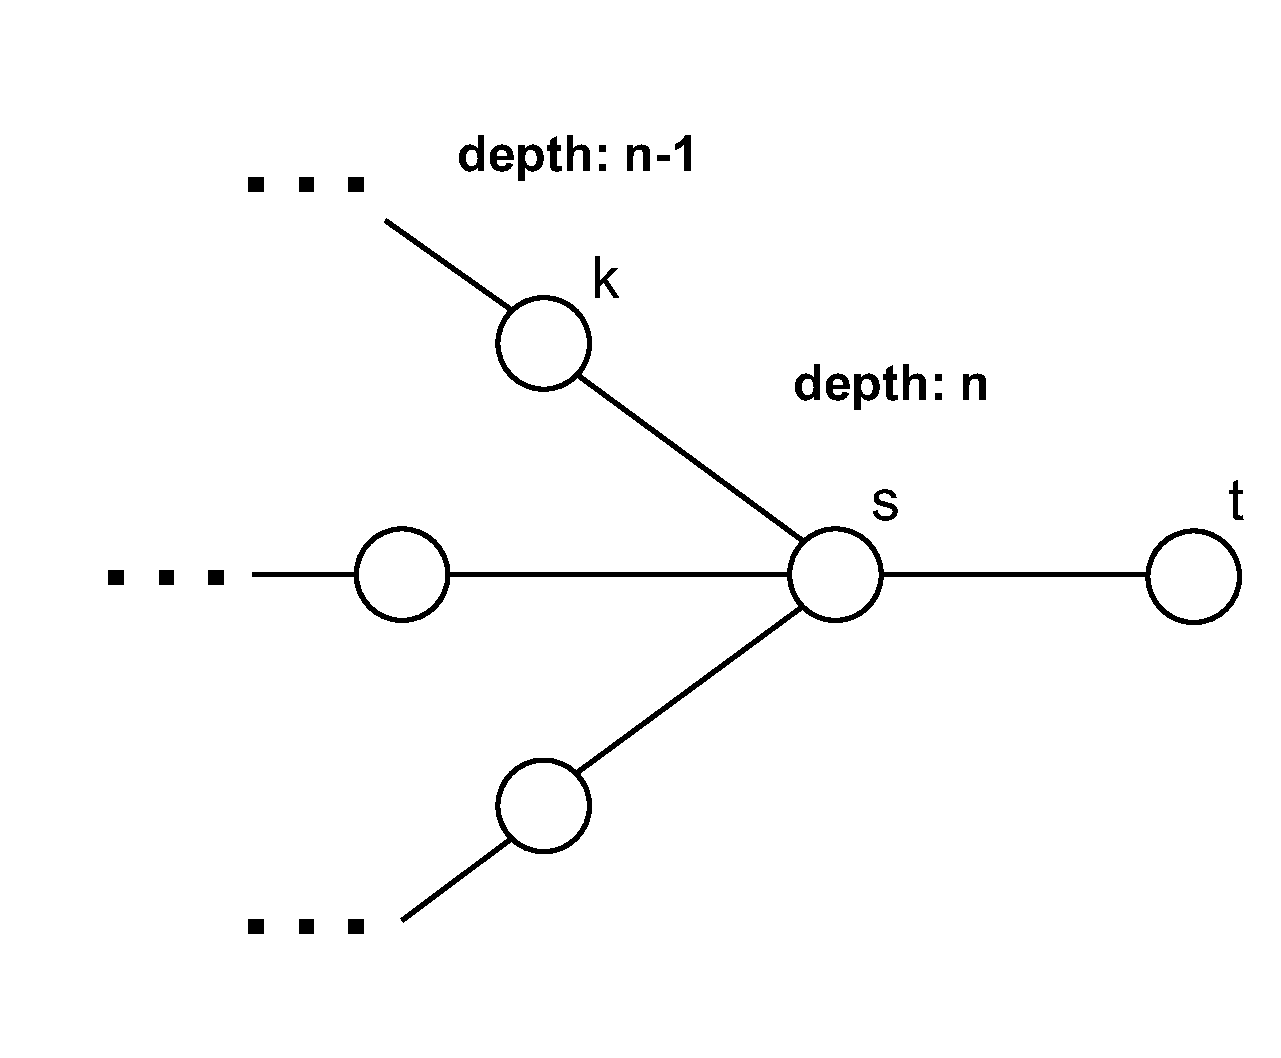
\includegraphics[width=0.4\columnwidth]{5b.pdf}
  \vspace{-0.1cm}
  \caption{Induction from depth $n-1$ to $n$.}
  \label{f:5b}
\end{figure}
%
Assume the equation holds for trees with depth up to $n-1$. For a tree with depth $n$,
suppose a node (node $\s{s}$ in Figure~\ref{f:5b}) on a path with length $n$
were to send the message out (to a hypothetical node $\s{t}$ in Figure~\ref{f:5b}),
the message can be written as
\begin{align*}
	m_{\s{s}\to\s{t}}^*(x_t) &= \sum_{x_s}\phi(x_s)\psi(x_s, x_t)\prod_{k\in \partial s \backslash\{t\}}m^*_{k\to s}(x_s)\\
	&=\sum_{x_s}\phi(x_s)\psi(x_s, x_t)\prod_{k\in \partial s \backslash\{t\}}\sum_{\{x_v|v\in T_k\}}\psi(x_k, x_s)\prod_{v\in T_k}\phi(x_v)\prod_{(i,j)\in T_k}\psi(x_i, x_j)\\
	&=\sum_{\{x_v|v\in T_s\}}\phi(x_s)\psi(x_s, x_t)\prod_{k\in \partial s \backslash\{t\}}\psi(x_k, x_s)\prod_{v\in T_k}\phi(x_v)\prod_{(i,j)\in T_k}\psi(x_i, x_j),
\end{align*}
where we can move the summation because $x_v$ are on the singleton potential. Further merging terms, we have
\begin{align*}
&\sum_{\{x_v|v\in T_s\}}\phi(x_s)\psi(x_s, x_t)\prod_{k\in \partial s \backslash\{t\}}\psi(x_k, x_s)\prod_{v\in T_k}\phi(x_v)\prod_{(i,j)\in T_k}\psi(x_i, x_j)\\
= &\sum_{\{x_v|v\in T_s\}}\psi(x_s, x_t)\prod_{k\in \partial s \backslash\{t\}}\psi(x_k, x_s)\prod_{v\in T_s}\phi(x_v)\prod_{(i,j)\in T_k}\psi(x_i, x_j)\\
= &\sum_{\{x_v|v\in T_s\}}\psi(x_s, x_t)\prod_{v\in T_s}\phi(x_v)\prod_{(i,j)\in T_v}\psi(x_i, x_j).
\end{align*}
Thus, by induction, the message passing fixed point $m^*$ satisfies the property. \qeds
\\

\noindent
(c) Since the marginal $\s{x}_s$ is proportional to summing other random variables in the potentials over the cliques, we have
\begin{align*}
	p(x_s) &\propto \sum_{\big\{x_v|v\in\mathscr{V}\backslash\{s\}\big\}}\prod_{v\in\mathscr{V}}\phi(x_v)\prod_{i,j\in\mathscr{E}}\psi(x_i, x_j)\\
	&=\phi(s) \sum_{\big\{x_v|v\in\mathscr{V}\backslash\{s\}\big\}}\prod_{v\in\mathscr{V}\backslash\{s\}}\phi(x_v)\prod_{i,j\in\mathscr{E}}\psi(x_i, x_j).
\end{align*}
%
Now we can slide the summation term inside the products, by skipping the irrelevant terms. Specially, we break down the neighboring nodes of $\s{s}$, 
%
\begin{align*}
	p(x_s) &\propto \phi(s) \prod_{t\in N(s)}\left[\sum_{\{x_v|v\in T_t\}}\psi(x_t, x_s)\prod_{v\in T_t}\phi(x_v)\prod_{i,j\in T_t}\psi(x_i, x_j)\right].
\end{align*}
Notice that we are able to separate the product term for edge potential to each
sub-tree $\prod_{i,j\in T_t}\psi(x_i, x_j)$, because there is no edge across the sub-trees (otherwise forming cycles); and $\psi(x_t, x_s)$ is singled out in the front as it is excluded from the sub-tree but existed originally in $\mathscr{E}$.

By part (b), we arrive that
\begin{align*}
	p(x_s) &\propto \phi(s) \prod_{t\in N(s)}m_{t\to s}^*(x_s).
\end{align*}\qeds
\\

\noindent
(d) Similar to (c), since the marginal on $\s{x}_s, \s{x}_t$ is proportional to summing other random variables in the potentials over the cliques, we have
\begin{align*}
	p(x_s, x_t) &\propto \sum_{\big\{s_v|v\in\mathscr{V}\backslash\{s,t\}\big\}}\prod_{v\in\mathscr{V}}\phi(x_v)\prod_{i,j\in\mathscr{E}}(x_i,x_j)\\
	&= \phi(x_s)\phi(x_t)\psi(x_s, x_t)
	\sum_{v\in T_s\backslash\{s\}}\left[\prod_{v\in T_s\backslash\{s\}}\phi(x_v)\prod_{i, j \in T_s}
	\psi(x_i,x_j)\right]
	\sum_{v\in T_t\backslash\{t\}}\left[\prod_{v\in T_t\backslash\{t\}}\phi(x_v)\prod_{i, j \in T_t}
	\psi(x_i,x_j)\right].
\end{align*}
Here, we can break the edge potential into two sub-trees because there is no edges across these two groups, otherwise cycles would be formed. Now, similar to (c), we can further expand to the neighbor nodes of $\s{s}$ and $\s{t}$ for message passing. Specially
\begin{align*}
	&\sum_{v\in T_s\backslash\{s\}}\left[\prod_{v\in T_s\backslash\{s\}}\phi(x_v)\prod_{i, j \in T_s}
	\psi(x_i,x_j)\right]\\
	=& \prod_{u\in N(s)\backslash\{t\}}\left[\sum_{x_v|v\in T_u}\psi(x_u, x_s)\prod_{v\in T_u}\phi(x_v)\prod_{i,j\in T_u}(x_i, x_j)\right],
\end{align*}
where edge potentials are further separated into each sub-tree, and the edge potentials that connects $x_u$ and $x_s$ are singled out in the front, as they are excluded from subtree $T_u$ but existed in $\mathscr{E}$.

Similarly, for the other half we have
\begin{align*}
	&\sum_{v\in T_t\backslash\{t\}}\left[\prod_{v\in T_t\backslash\{t\}}\phi(x_v)\prod_{i, j \in T_t}
	\psi(x_i,x_j)\right]\\
	=& \prod_{u\in N(t)\backslash\{s\}}\left[\sum_{x_v|v\in T_t}\psi(x_t, x_s)\prod_{v\in T_t}\phi(x_v)\prod_{i,j\in T_t}(x_i, x_j)\right].
\end{align*}

By part (b), we have
\begin{align*}
	p(x_s, x_t) &\propto \phi(x_s)\phi(x_t)\psi(x_s, x_t) \prod_{u\in N(s)\backslash\{t\}}m^*_{u\to s}(x_s) \prod_{v\in N(t)\backslash\{s\}}m^*_{v\to t}(x_t).
\end{align*}\qeds
\end{document}